\begin{frame}{Implementation}
    In order to run a schedulability analysis on the RTIC application,
    RAUK needs to fetch the following additional information
    \vspace{1em}
    \begin{itemize-size}{1em}
        \item Measure the WCET of all tasks
        \item Record a trace of the tasks in order to
        calculate the blocking time
    \end{itemize-size}     
\end{frame}

\begin{frame}{Implementation - Execution flow}
    \begin{itemize-size}{1em}
        \item Generate test vectors
        \item Replay and measure test vectors on hardware
        \item Calculate and determine if system is schedulable
    \end{itemize-size}
    
\end{frame}

\begin{frame}{Implementation - Generating tests}
    \begin{columns}
        \column{0.5\textwidth}
        \begin{block}{Generate test vectors}
            \begin{itemize-size}{1em}
                \item We build the RTIC application such that KLEE can run on it
                \item Generate tests targeting all possible execution paths using KLEE
                \item Task resources as symbolic values
                \item \textbf{ASSUMPTION:} At least one test vector generated for a task, should
                result in the WCET of that task!
            \end{itemize-size}  
        \end{block}

        \column{0.5\textwidth}
        \begin{figure}
            \centering
            
\includegraphics[scale=0.3]{pictures/softwaretesting.jpg}
        \end{figure}
    \end{columns}
\end{frame}

\begin{frame}{Implementation - Measure tests}
    \begin{block}{Replay the test vectors}
        \begin{itemize-size}{1em}
            \item Build the application such that we can test it on the target hardware
            \item Each test vector will be executed on the target hardware, by overwriting
            memory addresses and registers as necessary
            \item Set breakpoints at:
            \begin{itemize-size}{1em}
                \vspace{0.5em}
                \item When a task starts/ends
                \item When a task claims/releases a resource
            \end{itemize-size}
        \end{itemize-size}  
    \end{block}
\end{frame}

\begin{frame}{Implementation - Measure tests}
    \begin{columns}
        \column{0.5\textwidth} 
        \begin{block}{Replay the test vectors (contd.)}
            \begin{itemize-size}{1em}
                \item For each test vector, when hitting a breakpoint we record
                \begin{itemize-size}{1em}
                    \item Current clock cycle
                    \item What task is starting/ending or
                    \item Which resource is claimed or released
                \end{itemize-size}
                \item Finally we end up with a trace for that test vector
                \item Repeat until all test vectors have been measured 
            \end{itemize-size}  
        \end{block}

        \column{0.5\textwidth} 
        \begin{figure}
           \centering
            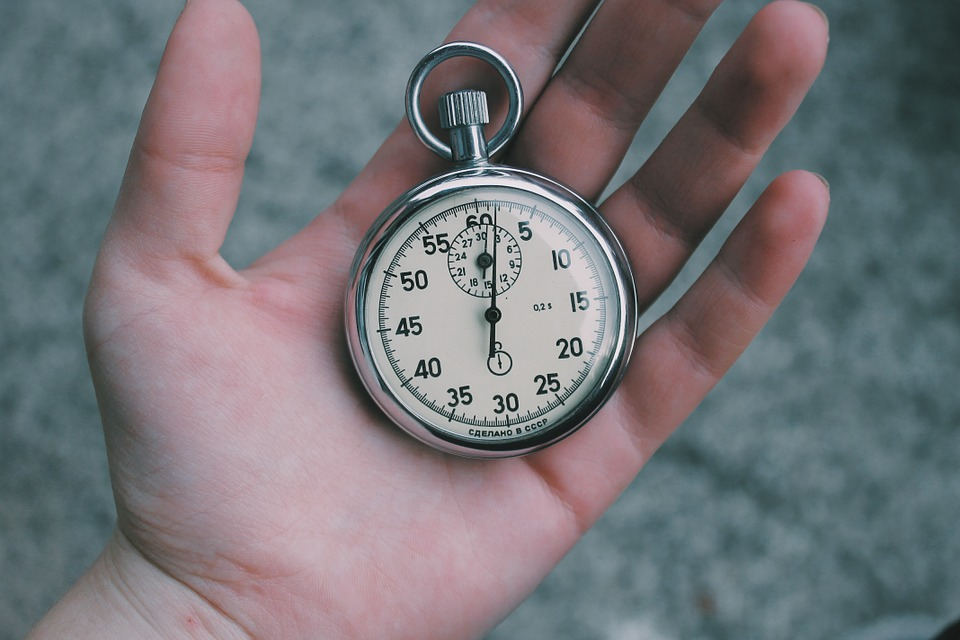
\includegraphics[scale=0.15]{pictures/stopwatch.jpg}
        \end{figure}
    \end{columns}
\end{frame}


\begin{frame}{Implementation}
    \begin{block}{Schedulability analysis}
        After recording the traces RAUK can
        \begin{itemize-size}{1em}
            \vspace{0.5em}
            \item Calculate the WCET for each trace
            \item Determine blocking times on all tasks using the traces
            \item Calculate WCRT for each trace
            \item Determine wheter the system is schedulable or not
        \end{itemize-size}  
    \end{block}
\end{frame}

\begin{frame}{Result}
    \begin{block}{Test setup}
        \begin{itemize-size}{1em}
            \item RTIC blinky application with a button to interrupt the LED
            \item Tested on an STM32 development board
            \item Deadline and period/inter-arrival time for each
            task given
            \item Tested with and without compiler optimizations
        \end{itemize-size}
    \end{block}
\end{frame}

\begin{frame}{Result}
    \begin{block}{Results}
        \begin{itemize-size}{1em}
            \item RAUK can successfully test, measure and
            run a schedulability analysis check without compiler optimizations
            \item RAUK has some limitations when running with compiler optimizations
            enabled
            \item Result compared with manual tracing of the test vectors
            \item RAUK adds some overhead to each measurement with and without
            optimizations
        \end{itemize-size}
    \end{block}
\end{frame}
